\section{INTRODUCCIÓN}

% TODO:
% Se hace MUY poco enfasis en la solucion a la ec. de movimiento. 
% La raiz cuadrada de lorentziana ni aparece

Un resonador microelectromecánico (MEMS) es una estructura mecánica
micrométrica cuyo movimiento se puede excitar y detectar eléctricamente. En
este trabajo se estudia el resonador A5, cuya parte móvil se encuentra entre
dos electrodos en forma de peine, como se muestra en la
Figura~\ref{fig:intro-a5}. Al moverse la estructura, cambia la capacitancia
entre los dientes de los peines. Esta variación permite detectar la
oscilación a partir de una señal eléctrica.

\begin{figure}[tb]
\centering
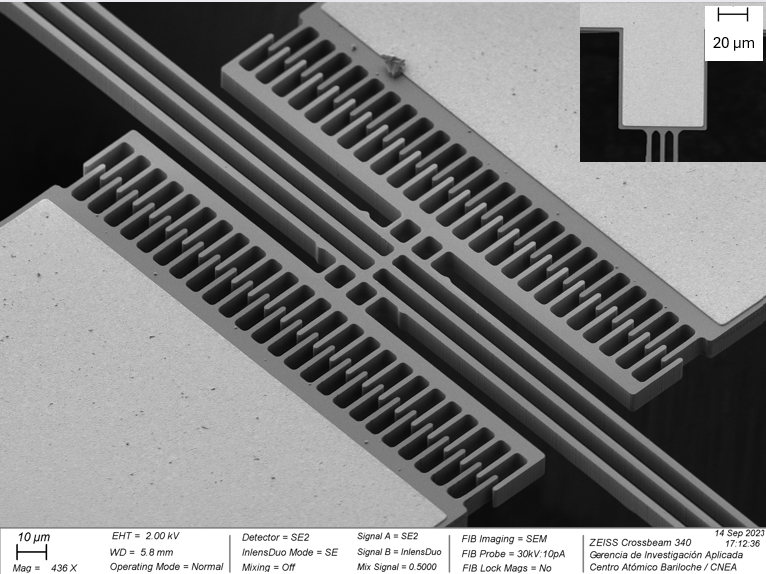
\includegraphics[width=.8\linewidth]{figuras/ImagenResonador.png}
% Micrografía SEM del resonador y sus extremos.
\caption{Micrografía del resonador A5. En el centro se ven las vigas de la
parte móvil y, por encima y por debajo, los electrodos en forma de peine.
La barra de escala corresponde a \SI{10}{\micro\metre}. En la parte superior derecha
se muestra el anclaje del resonador que conforma sus extremos.}
\label{fig:intro-a5}
\end{figure}

Para describir el movimiento cerca de una resonancia, se puede empezar por
considerar un solo modo de vibración. Si $x$ representa el desplazamiento
del modo, a pequeñas amplitudes la fuerza restauradora es aproximadamente
proporcional a $x$, un comportamiento de oscilador armónico al cual se lo identifica como régimen lineal. A mayores amplitudes, el estiramiento de las vigas hace
que esta aproximación deje de ser suficiente. Si se agrega un término
cúbico a la fuerza restauradora, se obtiene la ecuación de Duffing,
\begin{equation}
m\ddot{x}+b\dot{x}+kx+\alpha x^3
=F_0\cos(2\pi f_{\mathrm{exc}}t),
\label{eq:intro-duffing}
\end{equation}
\noindent donde $m$ es la masa efectiva del modo, $b$ es el coeficiente de
amortiguamiento, $k$ es la rigidez lineal y $\alpha$ es el coeficiente
cúbico. La fuerza periódica tiene amplitud $F_0$ y frecuencia
$f_{\mathrm{exc}}$.

En el régimen lineal, la frecuencia de oscilación libre es prácticamente
independiente de la amplitud y vale $f_0\simeq\sqrt{k/m}/(2\pi)$ si el
amortiguamiento es débil. En este régimen, el cuadrado de la amplitud de
respuesta cerca de $f_0$ sigue un perfil lorentziano. Por lo tanto, el
módulo de respuesta es proporcional a la raíz cuadrada de ese perfil.
Cuando $\alpha>0$, la frecuencia aumenta con la
amplitud $A$ de la oscilación. Para corrimientos pequeños, el aumento es
aproximadamente proporcional a $A^2$. Este comportamiento se conoce como
endurecimiento. Al barrer la frecuencia de excitación con $F_0$ fijo, la
curva de respuesta se inclina hacia frecuencias mayores, como se muestra
en la Figura~\ref{fig:intro-duffing}. Para una excitación suficientemente
grande, pueden coexistir dos amplitudes estables a una misma frecuencia.
La amplitud medida depende entonces del sentido del barrido, lo que da
lugar a la histéresis.

\begin{figure}[tb]
\centering
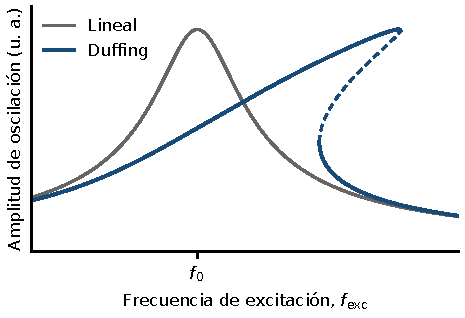
\includegraphics[width=.8\linewidth,trim=6bp 0 -6bp 0,clip=false]{figuras/respuesta_duffing.pdf}
\caption{Respuesta de un oscilador forzado cerca de la resonancia lineal
$f_0$. Se comparan el caso lineal y el caso con endurecimiento para una
misma amplitud de fuerza. El tramo discontinuo indica soluciones inestables.
En el intervalo donde se superponen las dos ramas estables, la respuesta
depende del sentido del barrido. Las curvas son teóricas.}
\label{fig:intro-duffing}
\end{figure}

El corrimiento de la frecuencia con la amplitud permite que el modo
principal se acerque a una relación de frecuencias simple con otro modo de
la misma estructura. Por ejemplo, si $f_1$ es la frecuencia de oscilación
del modo principal y $f_3$ la de un modo superior, la condición
$f_3\simeq 3f_1$ corresponde a una resonancia interna 1:3 cuando el
acoplamiento entre ambos permite el intercambio de energía.

Durante la excitación, el modo de mayor frecuencia puede almacenar parte
de la energía que recibe del modo principal. Al apagar la fuerza externa,
esa energía puede volver al modo principal y mantener casi constantes su
amplitud y su frecuencia durante un breve intervalo de tiempo, llamado tiempo de coherencia. En ese intervalo,
el intercambio de energía puede dar lugar a bandas laterales, que son
picos a ambos lados de la frecuencia principal en el
espectro~\cite{chen-2017}.

El objetivo de este trabajo es caracterizar la respuesta del resonador A5
desde el régimen lineal hasta el no lineal y evaluar si presenta señales
compatibles con una resonancia interna 1:3. Para ello se estudia cómo se
desplaza el pico al variar la amplitud de excitación y se compara la
respuesta al barrer la frecuencia en ambos sentidos. También se registra
la oscilación libre tras apagar la excitación (\textit{ringdown}). En estos
registros se analiza si el decaimiento comienza de inmediato o si existe
tiempo de coherencia.
